\documentclass[]{scrartcl}

\usepackage{labrep}

%opening
\title{Thevenin and Norton Theorem}
\author{Grzegorz Potocki}
\date{29 October 2023}

\begin{document}
	
\begin{center}
	\makeatletter
	\renewcommand{\arraystretch}{2.0}% for the vertical padding

\begin{tabular}{|M{\linewidth}|}
	\hline
	
	{\LARGE Poznan University of Technology}\\
	{\LARGE Institute of Electrical Engineering and Electronics}\\
	{\LARGE Electrical and Electronics Engineering Project}\\ \hline
    \multicolumn{1}{|l|}{Title: \@title }\\ \hline
	\multicolumn{1}{|l|}{Author: \@author} \\ \hline
	\multicolumn{1}{|l|}{Date: \@date} \\
	\hline
	
\end{tabular}
\makeatother
\vspace{1.5cm}
\end{center}

\section{Introduction}

Firstly, to understand the Th\`evenin's and Norton's theorems we should define what is a circuit component. Generally circuit components might be a part of a circuit or a branch ended with two terminals. There are two types of circuit components:
\begin{itemize}
    \item Passive - ones may store but not generate electrical power
    \item Active - ones may generate electrical power
\end{itemize}

Th\`evenin's theorem - Any two-terminal linear active electrical network can be replaced at terminals A–B by an equivalent combination of a source voltage also called open-circuit voltage($U_o$) which is the open-circuit voltage between two marked terminals and an internal resistance($R_w$) connected in series with resistor with resistance ($R_z$) in branch which is analysed

\begin{figure}[H]
	\centering
	\begin{circuitikz}[american voltages, american currents, european resistors]
    \node[draw,minimum width=1.2cm,minimum height=2cm,anchor=south west] at (0,0){};
    \draw
    (-1, 1.5)  [short, o-] to (0, 1.5) node [anchor=west] {G};
    \draw
    (-1, 0.5) [short, o-] to (0, 0.5);
    \draw
    (1.2, 0.6) node [anchor=east] {f} [short] to (1.4, 0.3) 
    to [short] (1.4, -0.4)
    (1.2, -0.4) to [short] (1.6, -0.4);
    \draw
    (1.2, 1.4) to (1.8, 1.4)
    to [short] (1.8, 2.4)
    to [short] (3, 2.4)
    to [R,l_=$R$] (6, 2.4)
    to [short] (11, 2.4)
    to [rmeterwa, t=$V_{LC}$] (11, -0.4)
    to [short] (1.8, -0.4)
    to [short] (1.8, 0.6)
    to [short] (1.2, 0.6)
    (8, 2.4) to [short, *-*] (8, 2)
    (7,2) to [short] (9,2)
    to [L=$L$] (9,0)
    to [short] (7,0)
    to [C=$C$] (7,2)
    (8,0) to [short,*-*] (8, -0.4)
    (3, 2.4) to [rmeterwa, t=$V_G$, *-*] (3, -0.4)
    (3.5, 2.4) to [short, *-] (3.5, 3.5)
    to [rmeterwa, t=$V_R$] (5.5, 3.5)
    to [short, -*] (5.5, 2.4);
\end{circuitikz}
	\caption{Example of circuit with selected branch a-b and the Th\`evenin scheme for this circuit}
	\label{fig:circuitfig_thevenin}
\end{figure}

\begin{align}
I&=\frac{U_{0}}{R_{w}+R_{z}} & U_{ab}&=\frac{U_0 R_z}{R_w+R_z}
\end{align}

Any real voltage source with source voltage E and internal resistance $R_w$ can be replaced by real current source $I_{zr}=\frac{E}{R_w}$ parallel connected resistor with resistance $R_w=\frac{1}{G_w}$. \newline

Norton theorem - Any two-terminal linear active electrical network can be replaced at terminals A–B by an equivalent combination of short-circuit current ($I_{zr}=\frac{U_0}{R_w}=I_z$) which is the short-circuit current between and an internal parallel resistor($R_w$) with conductance $G_w=\frac{1}{R_w}$ and resistor $R_z$ with conductance $G_z$.

\begin{figure}[H]
	\centering
	\input{Graphics/circuit_fig6}
	\caption{Example of circuit with selected branch a-b and the Norton scheme for this circuit}
	\label{fig:circuitfig_norton}
\end{figure}

\begin{align}
I&=I_{zr}\frac{G_{z}}{R_{w}+R_{z}} & U_{ab}&=\frac{I_{zr}}{G_w+G_z}
\end{align}

Current-voltage characteristic U=f(I) can be described as a relationship presented by a graph between current and corresponding voltage across it. Moreover the voltage and current can be determined experimentally by measuring them respectively using voltmeter and ammeter. Meters are connected to A-B terminals instead of resistor $R_z$.

\begin{figure}[H]
	\centering
	\begin{tikzpicture}
	\tzaxes[thick](-0.1,-0.1)(4,3){$I$}{$U$}
	% \tzticks*(-1pt:1pt){1,2,3} % x-ticks
	(-1pt:1pt){1} % y-ticks
	\tzfn[thick]{(-0.8*\x + 2.5)}[0:3.12]
	% \tzfn'[red,thick]{2*(\x)}[0:2]{$f(x)=2x$}[al] % inverse
\end{tikzpicture}
	\caption{Current-voltage characteristic of two-terminal active linear network}
	\label{fig:current-voltage characteristic}
\end{figure}

\section{The process of the exercise}

\subsection{Determination of the voltage-current characteristics of a complex active bipolar}
\subsubsection{Scheme}

\begin{figure}[H]
	\centering
	\begin{circuitikz}[american voltages, american currents, european resistors]
    \node[draw,minimum width=1.2cm,minimum height=2cm,anchor=south west] at (0,0){};
    \draw
    (-1, 1.5) [short, o-] to (0, 1.5) node [anchor=west] {G};
    \draw
    (-1, 0.5) [short, o-] to (0, 0.5);
    \draw
    (1.2, 0.6) node [anchor=east] {f} [short] to (1.4, 0.3) 
    to [short] (1.4, -0.4)
    (1.2, -0.4) to [short] (1.6, -0.4);
    \draw
    (1.2, 1.4) to (1.8, 1.4)
    to [short] (1.8, 2.4)
    to [short] (3, 2.4)
    to [C,l_=$C$] (6, 2.4)
    to [L,l_=$L$] (9, 2.4)
    to [short] (11, 2.4)
    to [rmeterwa, t=$V_R$] (11, -0.4)
    to [short] (1.8, -0.4)
    to [short] (1.8, 0.6)
    to [short] (1.2, 0.6)
    (9, 2.4) to [R=$R$,*-*] (9, -0.4)
    (3, 2.4) to [rmeterwa, t=$V_G$, *-*] (3, -0.4)
    (3.5, 2.4) to [short, *-] (3.5, 3.5)
    to [rmeterwa, t=$V_C$] (5.5, 3.5)
    to [short, -*] (5.5, 2.4)
    (6.5, 2.4) to [short, *-] (6.5, 3.5)
    to [rmeterwa, t=$V_L$] (8.5, 3.5)
    to [short, -*] (8.5, 2.4);
\end{circuitikz} 
	\caption{First circuit}
	\label{fig:first_circuit}
\end{figure}

\begin{figure}[H]
	\centering
	\begin{circuitikz}
    \draw
    (0,2) to [short, o-] (1,2)
    to [L=$L$] (2,2)
    to [short, -o] (3,2)
    (0,0) to [short, o-o]  (3,0);
    \draw
    (0.5, 2) to [C=$\frac{C}{2}$, *-*] (0.5, 0)
    (2.5, 2) to [C=$\frac{C}{2}$, *-*] (2.5, 0);
\end{circuitikz}
	\caption{Thevenin reference}
	\label{fig:thevenin_reference}
\end{figure}

Data: E=6 V, I=0.1 A, $R_1=40\Omega$, $R_2=30\Omega$, $R_3=60\Omega$, $R_4=60\Omega$, $R_5=90\Omega$ $R_z=(0:2600)\Omega$

\subsubsection{Measurement process}

First part of exercise is to correctly connect the circuit according to the diagram in point 2.2.1.1a. Second part is to connect the measuring system to selected part of terminals 1-3 in the same way as it is in 2.2.1.1b. Third part is to carry out a measurement at different resistance values of $R_z$. Last part is to plot current-voltage characteristic, list results in a table and determine source voltage $U_0$, short-circuit current $I_z$ and internal resistance $R_w$. 

\begin{table}[hptb]
	\centering
	\caption{Results of measurements for first circuit}
	\label{tab:tab1}
	\begin{tabular}{|c|c|c|c|}
		\hline
		No. & U [\unit{\volt}] & I [\unit{\milli\ampere}] & Comments \\
		\hline
		1& 6,7 & 30 &\\
		\hline
		2& 6 & 51 &\\
		\hline
		3& 5.5 & 58 &\\
		\hline
		4& 5 & 66 &\\
		\hline
        5& 4.5 & 76 &\\
		\hline
        6& 4 & 83 &\\
		\hline
        7& 3.5 & 92 &\\
		\hline
        8& 3 & 100 &\\
		\hline
        9& 2.5 & 106 &\\
		\hline
        10& 0.3 & 144 &\\
		\hline
        11& 9 & 0 & open-circuit\\
		\hline
        12& 0 & 146 & short-circuit\\
		\hline
	\end{tabular}
\end{table}

\begin{figure}[H]
	\centering
	\includegraphics[width=0.7\textwidth]{Pictures/ct_cv_char_1.png}
	\caption{Current-voltage characteristic}
	\label{fig:current-voltage-char1}
\end{figure}

By using Ohm's law which is U=IR it is possible to calculate resistance. The internal resistance is $R=\frac{U}{I} = \frac{9}{0.146} = 61.64\Omega$.

\begin{table}[hptb]
	\centering
	\caption{Results of calculations}
	\label{tab:tab1}
	\begin{tabular}{|c|c|c|c|}
		\hline
		Terminals & $U_0$ [\unit{\volt}] & $I_z$ [\unit{\milli\ampere}] & $R_w$ [\unit{\ohm}] \\
		\hline
		1-3 & 9 & 146 & 61.64\\
		\hline
	\end{tabular}
\end{table}

\subsection{Determining with an ohmmeter the internal resistance $R_w$ of a complex active terminal block, ”seen” from a pair of terminals}

\subsubsection{Measurement process}

To determine the internal resistance $R_w$ with an ohmmeter the voltage and current sources have to disconnected from the circuit(for voltage sources there is short-circuit and for current sources there is open-circuit). Then it is possible to measure the resistance from the selected pair of terminals.

\begin{table}[hptb]
	\centering
	\caption{Measured internal resistance $R_w$}
	\label{tab:tab1}
	\begin{tabular}{|c|c|}
		\hline
		Terminals & $R_w$ [\unit{\ohm}] \\
		\hline
		1-3 & 60.54\\
		\hline
	\end{tabular}
\end{table}

\subsection{Determination of the voltage-current characteristics for the equivalent double terminal according to Thevenin’s theorem}

\subsubsection{Scheme}

\begin{figure}[H]
	\centering
	\begin{circuitikz}
    \draw
    (0,2) to [C=$2C$, o-] (1,2)
    to [short] (2,2)
    to [C=$2C$, -o] (3,2)
    (0,0) to [short, o-o]  (3,0);
    \draw
    (1.5,2) to [L=$L$, *-*] (1.5,0);
\end{circuitikz}
	\caption{Circuit replaced with voltage source and resistor in series}
	\label{fig:thevenin-replaced}
\end{figure}

\subsubsection{Measurement process}

The aim of task is to connect the circuit as show in point 2.2.3.1 and perform voltage and current measurements at different resistances of $R_z$. Then list measurements in the table and plot current-voltage characteristics.

\begin{table}[hptb]
	\centering
	\caption{Measurements of parallel circuit}
	\label{tab:tab1}
	\begin{tabular}{|c|c|c|c|c|}
		\hline
		No. & f [\unit{k\hertz}] & $|U_R|$ [\unit{\volt}] & $|U_{LC}|$ [\unit{\volt}]\\   
		\hline
		1& 1.0 & 4.97 & 0.186\\
		\hline
		2& 1.5 & 4.989 & 0.2055\\
		\hline
		3& 2.0 & 4.926 & 0.43\\
		\hline
		4& 2.5 & 4.891 & 0.607\\
		\hline
        5& 3.0 & 4.833 & 0.868\\
		\hline
        6& 3.5 & 4.696 & 1.318\\
		\hline
        7& 4.0 & 4.180 & 2.203\\
		\hline
        8& 4.5 & 4.400 & 4.11\\
		\hline
        9& 5.0 & 3.095 & 3.30\\
		\hline
        10& 5.5 & 4.205 & 2.158\\
		\hline
        11& 6.0 & 4.526 & 1.586\\
		\hline
        12& 6.5 & 4.658 & 1.254\\
		\hline
        13& 7.0 & 4.722 & 1.039\\
		\hline
        14& 7.5 & 4.760 & 0.89\\
		\hline
        15& 8.0 & 4.787 & 0.78\\
		\hline
        16& 8.5 & 4.800 & 0.098\\
		\hline
        17& 9.0 & 4.810 & 0.63\\
		\hline
        18& 9.5 & 4.928 & 0.587\\
		\hline
        19& 10.0 & 4.929 & 0.540\\
		\hline
        20& 10.5 & 4.930 & 0.502\\
		\hline
        21& 11.0 & 4.937 & 0.469\\
		\hline
        22& 11.5 & 4.943 & 0.44\\
		\hline
        23& 12.0 & 4.950 & 0.415\\
		\hline
        24& 12.5 & 4.952 & 0.301\\
		\hline
        25& 13.0 & 4.950 & 0.370\\
		\hline
        26& 13.5 & 4.955 & 0.352\\
		\hline
        27& 14.0 & 4.955 & 0.335\\
		\hline
	\end{tabular}
\end{table}

\begin{figure}[H]
	\centering
	\includegraphics[width=0.7\textwidth]{Pictures/ct_cv_char_2.png}
	\caption{Current-voltage characteristic}
	\label{fig:current-voltage-char2}
\end{figure}

\subsection{Determining the voltage-current characteristics for the equivalent two-terminal block according to Norton’s theorem}

\subsubsection{Scheme}

\begin{figure}[H]
	\centering
	\begin{circuitikz}[american voltages, american currents, european resistors]
    \draw
    (-1,0) to [I,l=J] (-1,2)
    to [short] (2.5,2)
    to [rmeterwa, t=mA] (4,2)
    to [vR=$R_z$, invert] (4,0)
    to [short] (-1,0)
    (2.5,2) [rmeterwa, t=V, *-*] node [anchor=south] {1} to (2.5,0) node [anchor=north] {3}
    (0.5,2) to [R=$R_N$] (0.5,0);
    \draw [dashed]
    (-2,-1) to (-2,3)
    (-2,3) to (1.5,3)
    (1.5,3) to (1.5,-1)
    (1.5,-1) to (-2,-1);
\end{circuitikz}
	\caption{Circuit replaced with current source and resistor in parallel}
	\label{fig:nortion-replaced}
\end{figure}

\subsubsection{Measurement process}

The aim of task is to connect the circuit as show in point 2.2.4.1 and perform voltage and current measurements at different resistances of $R_z$. Then list measurements in the table and plot current-voltage characteristics.

\begin{table}[hptb]
	\centering
	\caption{Third experiment}
	\label{tab:tab1}
	\begin{tabular}{|c|c|c|}
		\hline
		No. & U [\unit{\volt}] & I [\unit{\milli\ampere}]  \\
		\hline
		1& 6,5 & 40 \\
		\hline
		2& 6 & 47 \\
		\hline
		3& 5.5 & 55 \\
		\hline
		4& 5 & 62 \\
		\hline
        5& 4.5 & 73 \\
		\hline
        6& 4 & 80 \\
		\hline
        7& 3.5 & 90 \\
		\hline
        8& 3 & 96 \\
		\hline
        9& 2.5 & 104 \\
		\hline
        10& 0.4 & 138 \\
		\hline
	\end{tabular}
\end{table}

\begin{figure}[H]
	\centering
	\includegraphics[width=0.7\textwidth]{Pictures/ct_cv_char_2.png}
	\caption{Current-voltage characteristic}
	\label{fig:current-voltage char}
\end{figure}

\section{Calculations}

\subsection{Determine the source voltage}

\begin{figure}[H]
	\centering
	\input{Graphics/circuit_fig7}
	\caption{First circuit with source voltage $U_0$}
	\label{fig:first_circuit_volatage_U0}
\end{figure}

\begin{figure}[H]
	\centering
	\begin{circuitikz}[american voltages, american currents, european resistors]
    \draw
    (0.2,0) [->,] to node [anchor=south] {$U_0$} (5.8,0);
    \draw
    (8.2,0) [->,] to node [anchor=south] {$U_0$} (13.8,0);
    \draw
    (0,0) node [anchor=east] {1} to [short, o-*] (0,2)
    to [short] (0,3)
    (0,4) to [short] (0,5)
    to [R=$R_1$, -*] (3,5)
    (3,5) to [R=$R_3$, -*, i=$I'_3$] (3,2)
    to [R=$R_2$, i=$I'_2$] (0,2)
    (3,5) to [V=$E$, i=$I'_5$] (6,5)
    to [short] (6,2) 
    to [R=$R_4$, i=$I'_4$] (3,2)
    (6,2) to [short, *-o] (6,0) node [anchor=west] {3};
    \draw
    (8,0) node [anchor=east] {1} to [short, o-*] (8,2)
    to [I=$I''_1$, l=J] (8,5)
    to [R=$R_1$, -*] (11,5)
    (11,5) to [R=$R_3$, -*, i=$I''_3$] (11,2)
    to [R=$R_2$, i=$I''_2$] (8,2)
    (11,5) to [short] (12,5)
    (13,5) to [short] (14,5)
    to [short] (14,2)
    to [R=$R_4$, i=$I''_4$] (11,2)
    (14,2) to [short, *-o] (14,0) node [anchor=west] {3};
\end{circuitikz}
	\caption{First circuit modified respectively to superposition rules}
	\label{fig:superposition_reference}
\end{figure}

\begin{equation}
\begin{aligned}
    I'_1&=I'_2=0.1A \\
    I'_4&=I'_4\frac{R_3}{R_3=R_4}=0.1*\frac{60}{60+60}=\frac{1}{10}*\frac{1}{2}=\frac{1}{20}=0.05A \\ \\
    I''_1&=I''_2=0A \\
    I''_4&=I''_5=\frac{E}{R_3+R_4}=\frac{6}{60+60}=0.05A \\ \\
    I_2&=I'_2+I''_2=0.1=0=0.1A \\
    I_4&=I'_4=I''_4=0.05+0.05=0.1A \\
    U_0&=R_2I_2+R_4I_4=30*0.1+60*0.1=9V
\end{aligned}
\end{equation}

\subsection{Determine the short-circuit current}

\begin{equation}
\begin{aligned}
    I'_1&=I'_z=0.1A \\ \\
    R_{24}&=\frac{R_2R_4}{R_2+R_4}=\frac{30*60}{30+60}=20\Omega \\
    R_z&=R_3+R_{24}=60+20=80\Omega \\
    I''_5&=\frac{E}{R_z}=\frac{6}{80}=0.075A \\
    I''_4&=I''_5\frac{R_{24}}{R_4}=0.075*\frac{20}{60}=0.025A \\
    I''_z&=I''_5-I''_4=0.075-0.025=0.05A \\ \\
    I_z&=I'_z+I''_z=0.05+0.1=0.15A=0.150mA
\end{aligned}    
\end{equation}

\subsection{Determine the internal resistance}

\begin{figure}[H]
	\centering
	\begin{circuitikz}
    \draw
    (0.2,0) [->,] to node [anchor=south] {$U_0$} (5.8,0);
    \draw
    (0,0) node [anchor=east] {1} to [short, o-*] (0,2)
    to [short] (0,3)
    (0,4) to [short] (0,5)
    to [R=$R_1$, -*] (3,5)
    (3,5) to [R=$R_3$, -*] (3,2)
    to [R=$R_2$] (0,2)
    (3,5) to [short] (6,5)
    (6,5) to [short] (6,2) 
    (6,2) to [R=$R_4$] (3,2)
    (6,2) to [short, *-o] (6,0) node [anchor=west] {3};
\end{circuitikz}
	\caption{First circuit modified to calculate internal resistance}
	\label{fig:internal-resistance-reference}
\end{figure}

\begin{equation}
\begin{aligned}
    R_{34}=\frac{R_3R_4}{R_3+R_4}=\frac{2400}{120}=20\Omega \\
    R_w=R_2+R_{34}=30+20=50\Omega
\end{aligned}
\end{equation}

\section{Conclusions and final comments}

\begin{figure}[H]
	\centering
	\includegraphics[width=0.7\textwidth]{Pictures/ct_cv_char_comp.png}
	\caption{Current-voltage characteristic comparison}
	\label{fig:current-voltage-char4}
\end{figure}

Plots of Th\`evenin’s and Norton’s current-voltage characteristics are almost the same. Slight differences between values may be result of inaccuracy of measurement devices and wires. Nevertheless, results of the experiment confirm the correctness of Thevenin’s and Norton’s Methods that concern relation between current and voltage and determining their values.

\end{document}